\documentclass[tikz,border=8pt]{standalone}
\usepackage[T1]{fontenc}
\usepackage{tikz}
\usetikzlibrary{arrows.meta,positioning,calc}

\begin{document}
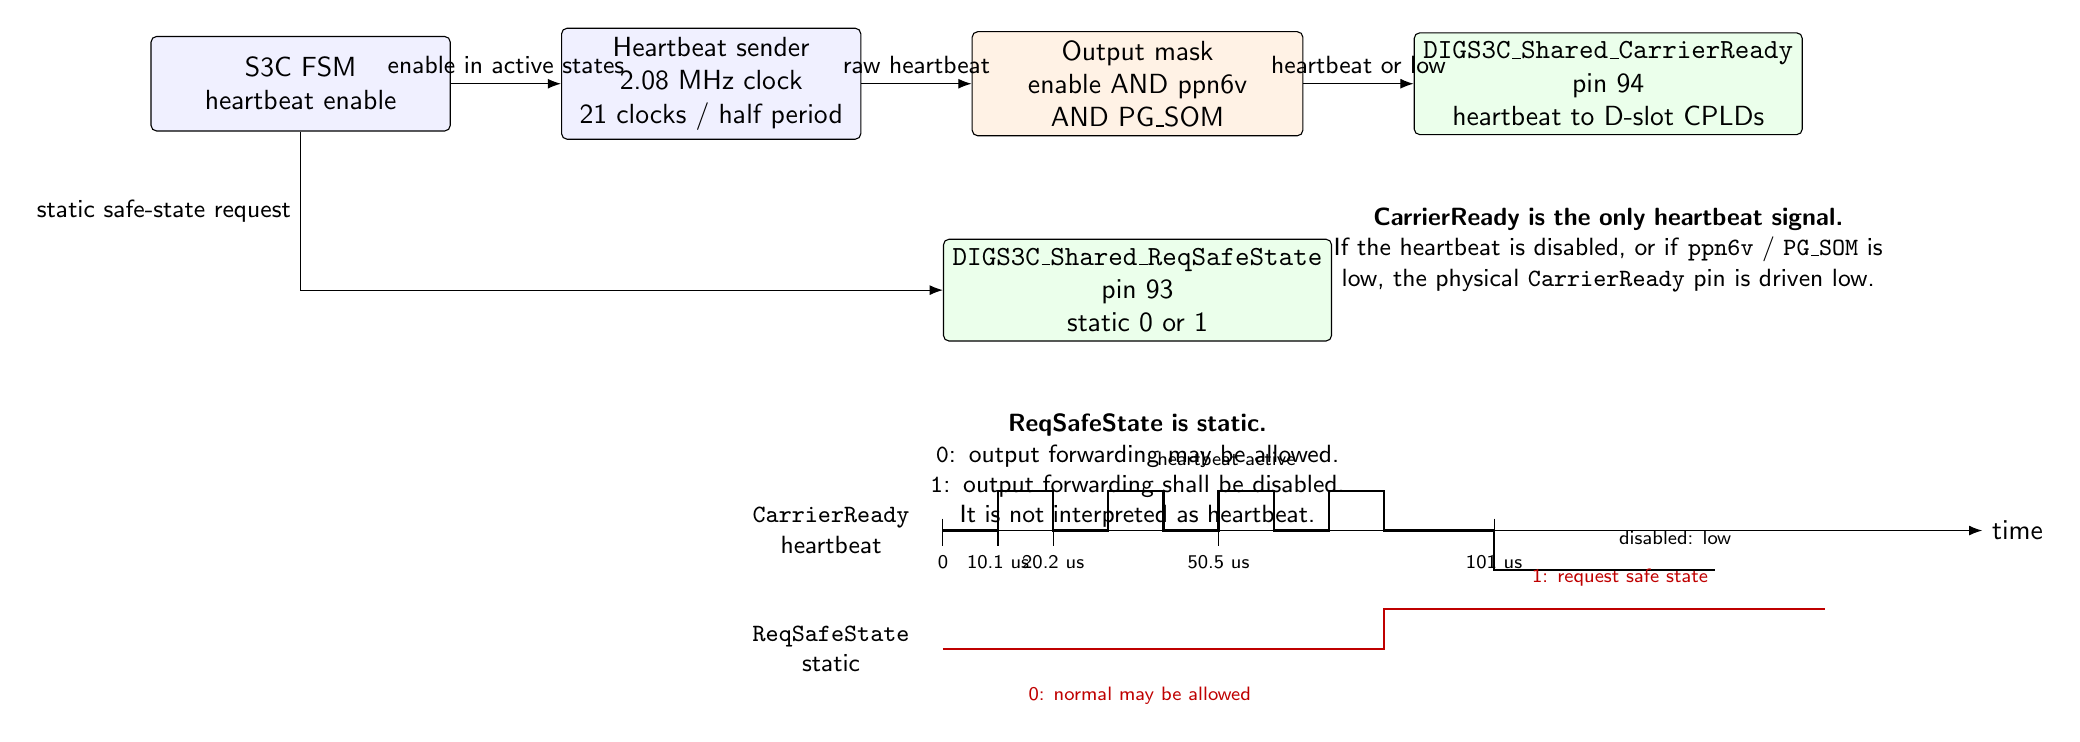
\begin{tikzpicture}[
  font=\sffamily,
  >=Latex,
  block/.style={draw, rounded corners=2pt, align=center, minimum height=12mm, minimum width=38mm, fill=blue!6},
  gate/.style={draw, rounded corners=2pt, align=center, minimum height=12mm, minimum width=42mm, fill=orange!10},
  signal/.style={draw, rounded corners=2pt, align=center, minimum height=10mm, minimum width=44mm, fill=green!8},
  note/.style={align=center, font=\sffamily\small},
  tinytext/.style={align=center, font=\sffamily\scriptsize},
  sig/.style={thick}
]

\node[block] (fsm) {S3C FSM\\heartbeat enable};
\node[block, right=14mm of fsm] (sender) {Heartbeat sender\\2.08 MHz clock\\21 clocks / half period};
\node[gate, right=14mm of sender] (mask) {Output mask\\enable AND ppn6v\\AND PG\_SOM};
\node[signal, right=14mm of mask] (carrier) {\texttt{DIGS3C\_Shared\_CarrierReady}\\pin 94\\heartbeat to D-slot CPLDs};

\node[signal, below=13mm of mask] (reqsafe) {\texttt{DIGS3C\_Shared\_ReqSafeState}\\pin 93\\static 0 or 1};

\draw[->] (fsm) -- node[above,note] {enable in active states} (sender);
\draw[->] (sender) -- node[above,note] {raw heartbeat} (mask);
\draw[->] (mask) -- node[above,note] {heartbeat or low} (carrier);
\draw[->] (fsm.south) |- node[pos=.25,left,note] {static safe-state request} (reqsafe.west);

\node[note, below=8mm of carrier, text width=70mm] {
\textbf{CarrierReady is the only heartbeat signal.}\\
If the heartbeat is disabled, or if \texttt{ppn6v} / \texttt{PG\_SOM} is low, the physical
\texttt{CarrierReady} pin is driven low.
};

\node[note, below=8mm of reqsafe, text width=72mm] {
\textbf{ReqSafeState is static.}\\
\texttt{0}: output forwarding may be allowed.\\
\texttt{1}: output forwarding shall be disabled.\\
It is not interpreted as heartbeat.
};

\coordinate (t0) at ($(reqsafe.south west)+(0,-24mm)$);
\draw[->] (t0) -- ++(132mm,0) node[right] {time};
\node[note, anchor=east] at ($(t0)+(-3mm,0mm)$) {\texttt{CarrierReady}\\heartbeat};
\node[note, anchor=east] at ($(t0)+(-3mm,-15mm)$) {\texttt{ReqSafeState}\\static};

\draw[sig] ($(t0)+(0,0)$)
  -- ++(7mm,0) -- ++(0,5mm) -- ++(7mm,0) -- ++(0,-5mm)
  -- ++(7mm,0) -- ++(0,5mm) -- ++(7mm,0) -- ++(0,-5mm)
  -- ++(7mm,0) -- ++(0,5mm) -- ++(7mm,0) -- ++(0,-5mm)
  -- ++(7mm,0) -- ++(0,5mm) -- ++(7mm,0) -- ++(0,-5mm)
  -- ++(14mm,0)
  -- ++(0,-5mm) -- ++(28mm,0);
\node[tinytext, anchor=south] at ($(t0)+(36mm,7mm)$) {heartbeat active};
\node[tinytext, anchor=south] at ($(t0)+(93mm,-3mm)$) {disabled: low};

\draw[sig, red!75!black] ($(t0)+(0,-15mm)$) -- ++(56mm,0)
  -- ++(0,5mm) -- ++(56mm,0);
\node[tinytext, red!75!black] at ($(t0)+(25mm,-21mm)$) {0: normal may be allowed};
\node[tinytext, red!75!black] at ($(t0)+(86mm,-6mm)$) {1: request safe state};

\foreach \x/\lab in {0/0,7/10.1 us,14/20.2 us,35/50.5 us,70/101 us} {
  \draw ($(t0)+(\x mm,1.5mm)$) -- ($(t0)+(\x mm,-2mm)$);
  \node[tinytext, anchor=north] at ($(t0)+(\x mm,-2mm)$) {\lab};
}

\end{tikzpicture}
\end{document}
